%!TEX root = ./Paper.tex

\section{Case Studies Irregular Gridshells}

\subsection{Further optimisation allowing variation on the segments length}

A further optimisation can also be achieved by allowing the distance between grid nodes to vary, reducing thus the curvature on the grid locally and globally. A spherical calotte of 15m diameter and 10m height has been firstly optimised, with constant segment length (regular gridshell) and a starting angle between profiles of $67.5^\circ$, and afterwards  by letting the segment lengths progressively differ (irregular gridshell). 

On the case of the calotte with regular mesh, due to the characteristic polar singularities of the spheres, strong local concentrations of curvature can be observed. By letting the mesh size vary, the segment lengths become shorter on the poles and the also typical alignment in S of the grid tends to disappear (see Fig.~\ref{fig:SphereIrregular}).

\begin{figure}[t]
\centering
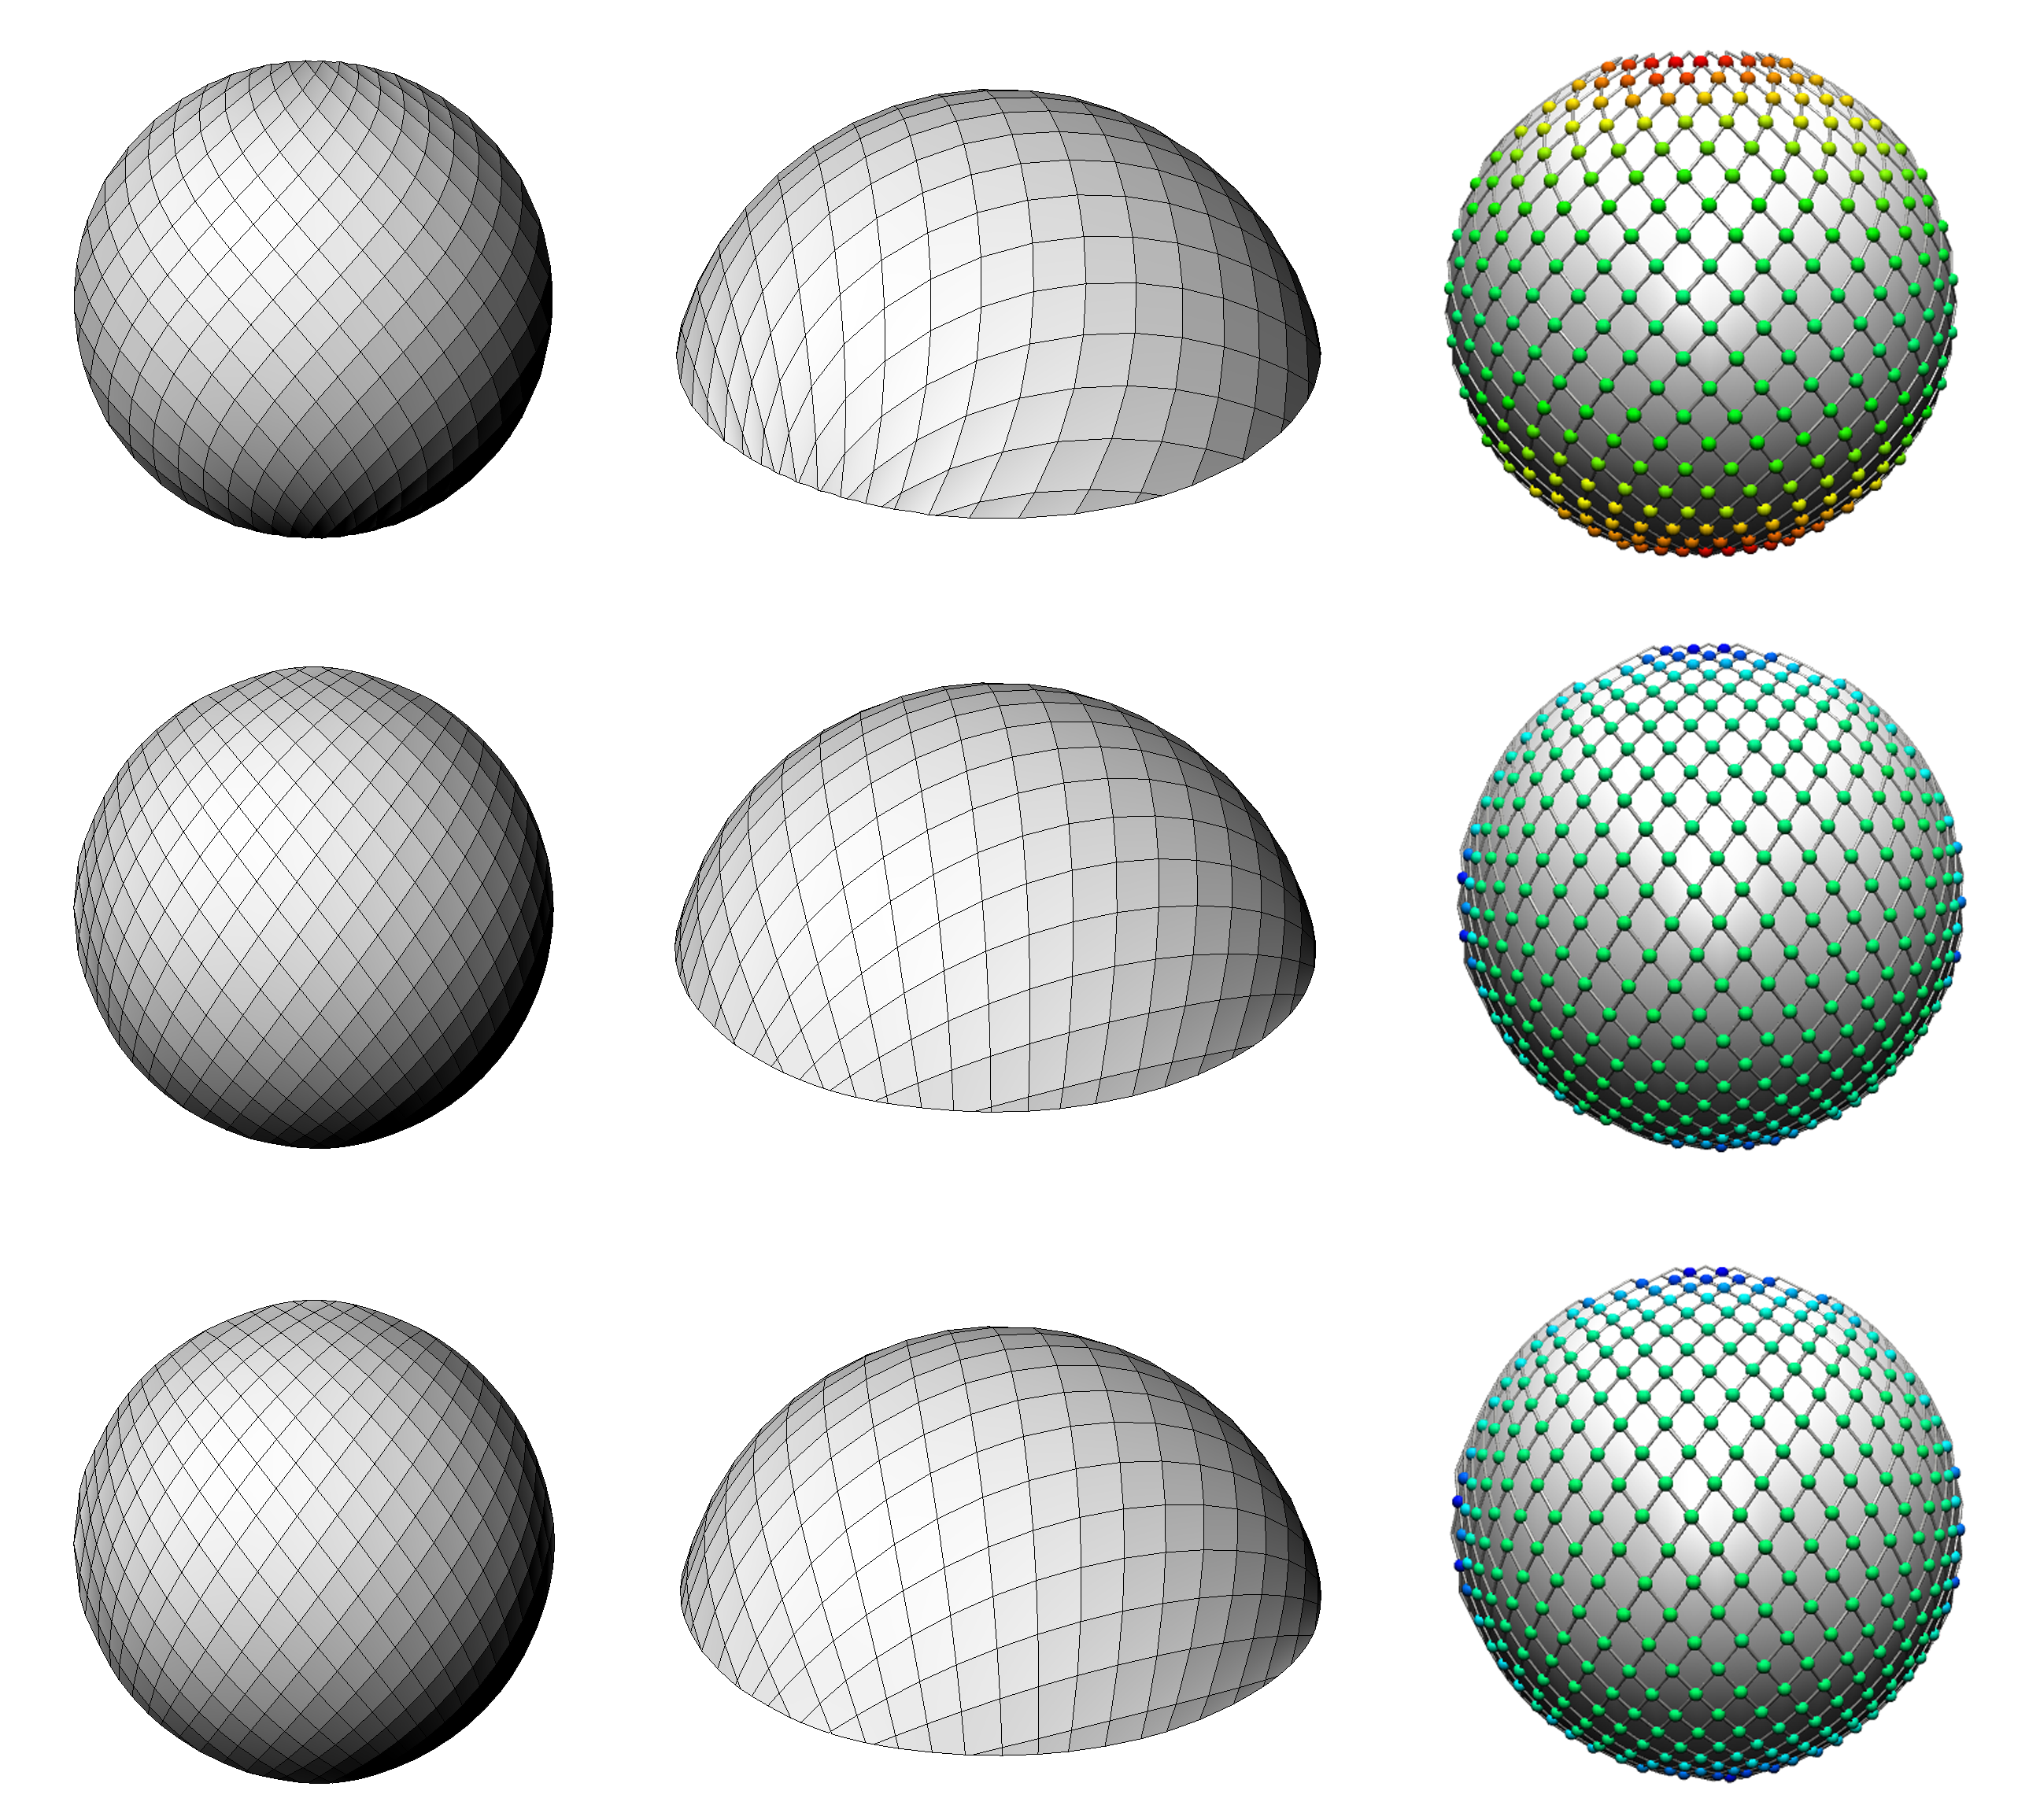
\includegraphics[width=0.80\linewidth]{images/CaseStudies_Irregular/SphereIrregular.png}
\caption{Optimisation of a spherical calotte with regular and irregular meshes. With a maximum variation of the segment length of 0.40m (middle) and 0.50m (bottom), the mean curvature of the grid could be reduced up to 83\% and 77\% respectively.}
\label{fig:SphereIrregular}
\end{figure}

\subsection{Practical application: The Flying Dome}

Elastic gridshells offer great advantages on temporary structures since the initially straight and afterwards elastically shaped profiles composing the grid allow rapid and cost-efficient production, transport and erection processes. For a temporary hanging 3D Projection Hemisphere (Flying Dome) of 10m diameter, an irregular elastic gridshell has been designed (see Fig.~\ref{fig:Renderings}). The project is a cooperation between the UdK Berlin, the TU Berlin, the Fraunhofer Institut FIRST and industrial partners and is planned to be built in Berlin in October 2012.

The structure consists in a hybrid construction composed of an irregular elastic gridshell between a double-layer membrane stabilized by underpressure (vacuum) of 0.08mbar. The profiles of the gridshell are made of GFK and have a tubular section of 20mm diameter and 3mm thickness.A third layer of profiles assures the bracing of the grid and activates its shear-bearing capacity. A PVC-coated polyester fabric and a PVC projection foil have been planned for the outer and inner membranes, respectively. The extremities of the bent profiles are fixed on a steel box ring of 100x100x4mm. The hemisphere hangs from the roof through four cables of 6mm diameter and is horizontally stabilized by other four cables of 3mm diameter. The total weight of the structure is approximately 1.3 tons.

\begin{figure}[ht]
\centering
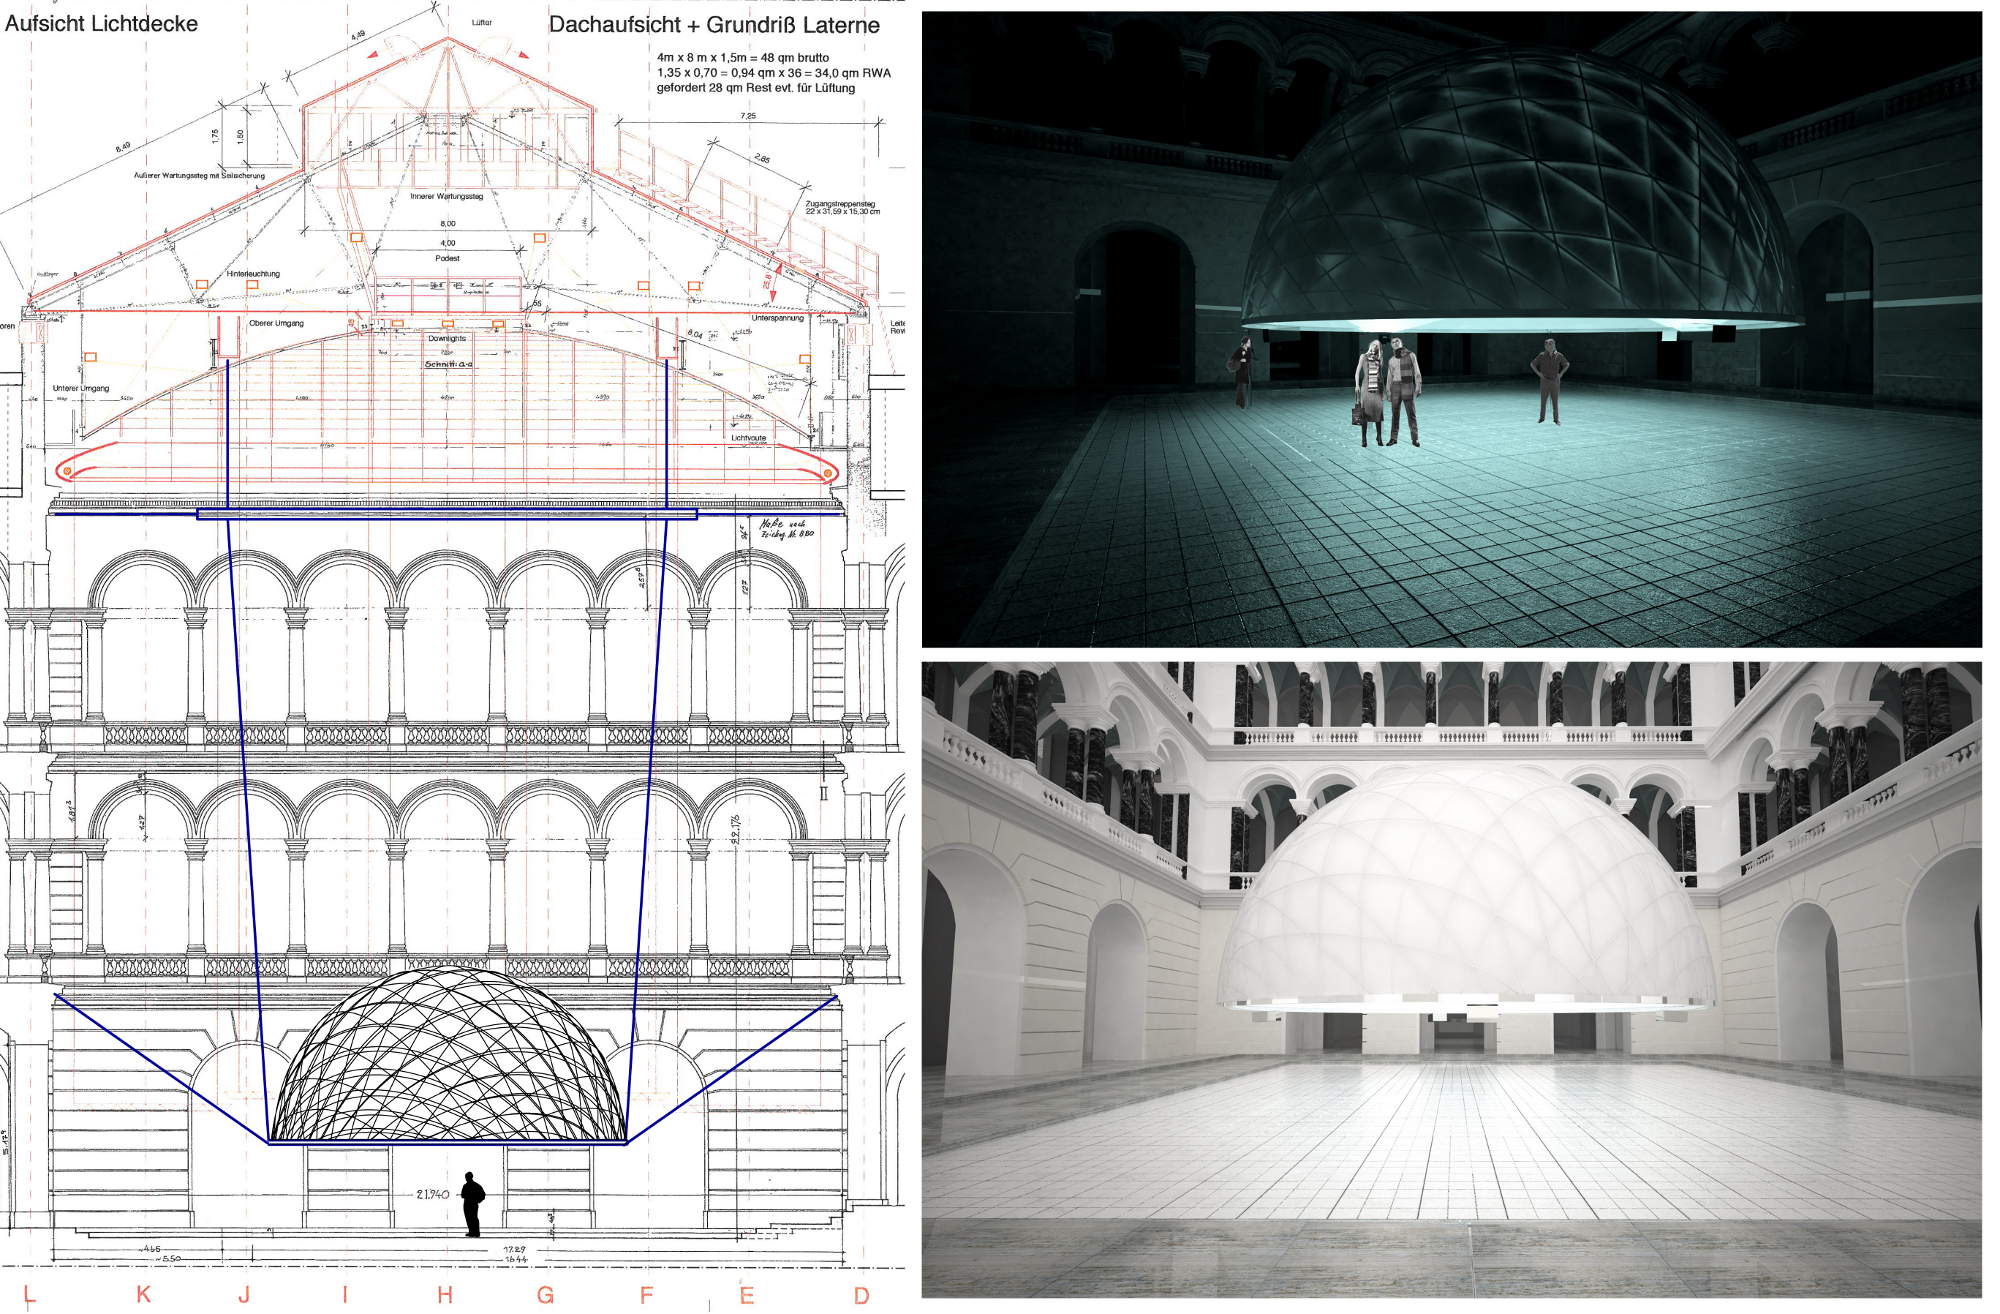
\includegraphics[width=1.0\linewidth]{images/Renderings_Modell/Renderings_lowres.png}
\caption{Front view and renderings of the Flying Dome}
\label{fig:Renderings}
\end{figure}

An irregular mesh was chosen in order to minimise the profiles curvature (the maximum curvature could be reduced up to 80% compared to the regular gridshell) and to obtain a more interesting arrangement of the grid pattern. Physical modelling was used to analyse the visual effects (see Fig.~\ref{fig:Modell}). 

\begin{figure}[ht]
\centering
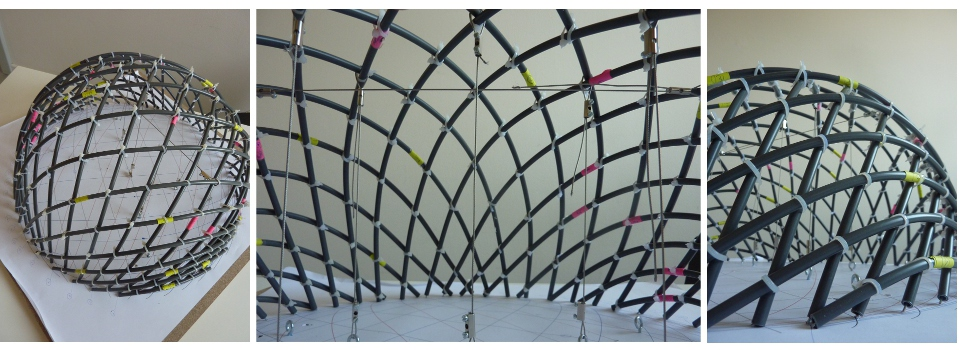
\includegraphics[width=1.0\linewidth]{images/Renderings_Modell/Modell.JPG}
\caption{Physical modelling of the Flying Dome to analyse the visual effects of the irregular mesh}
\label{fig:Modell}
\end{figure}

Contrary to regular grids, grids with irregular meshes cannot be completely deployed and can only be partially pre-assembled. The two profile layers will be joined and bent in a progressive process in order not to exceed the maximum allowable curvature during the erection of the structure. By means of FEA, the assembling process of the hemisphere has been simulated and the maximum stresses during the shaping of the grid and by underpressure loading have been controlled (see Fig.~\ref{fig:FEMGlobal}). 

\begin{figure}[ht]
\centering
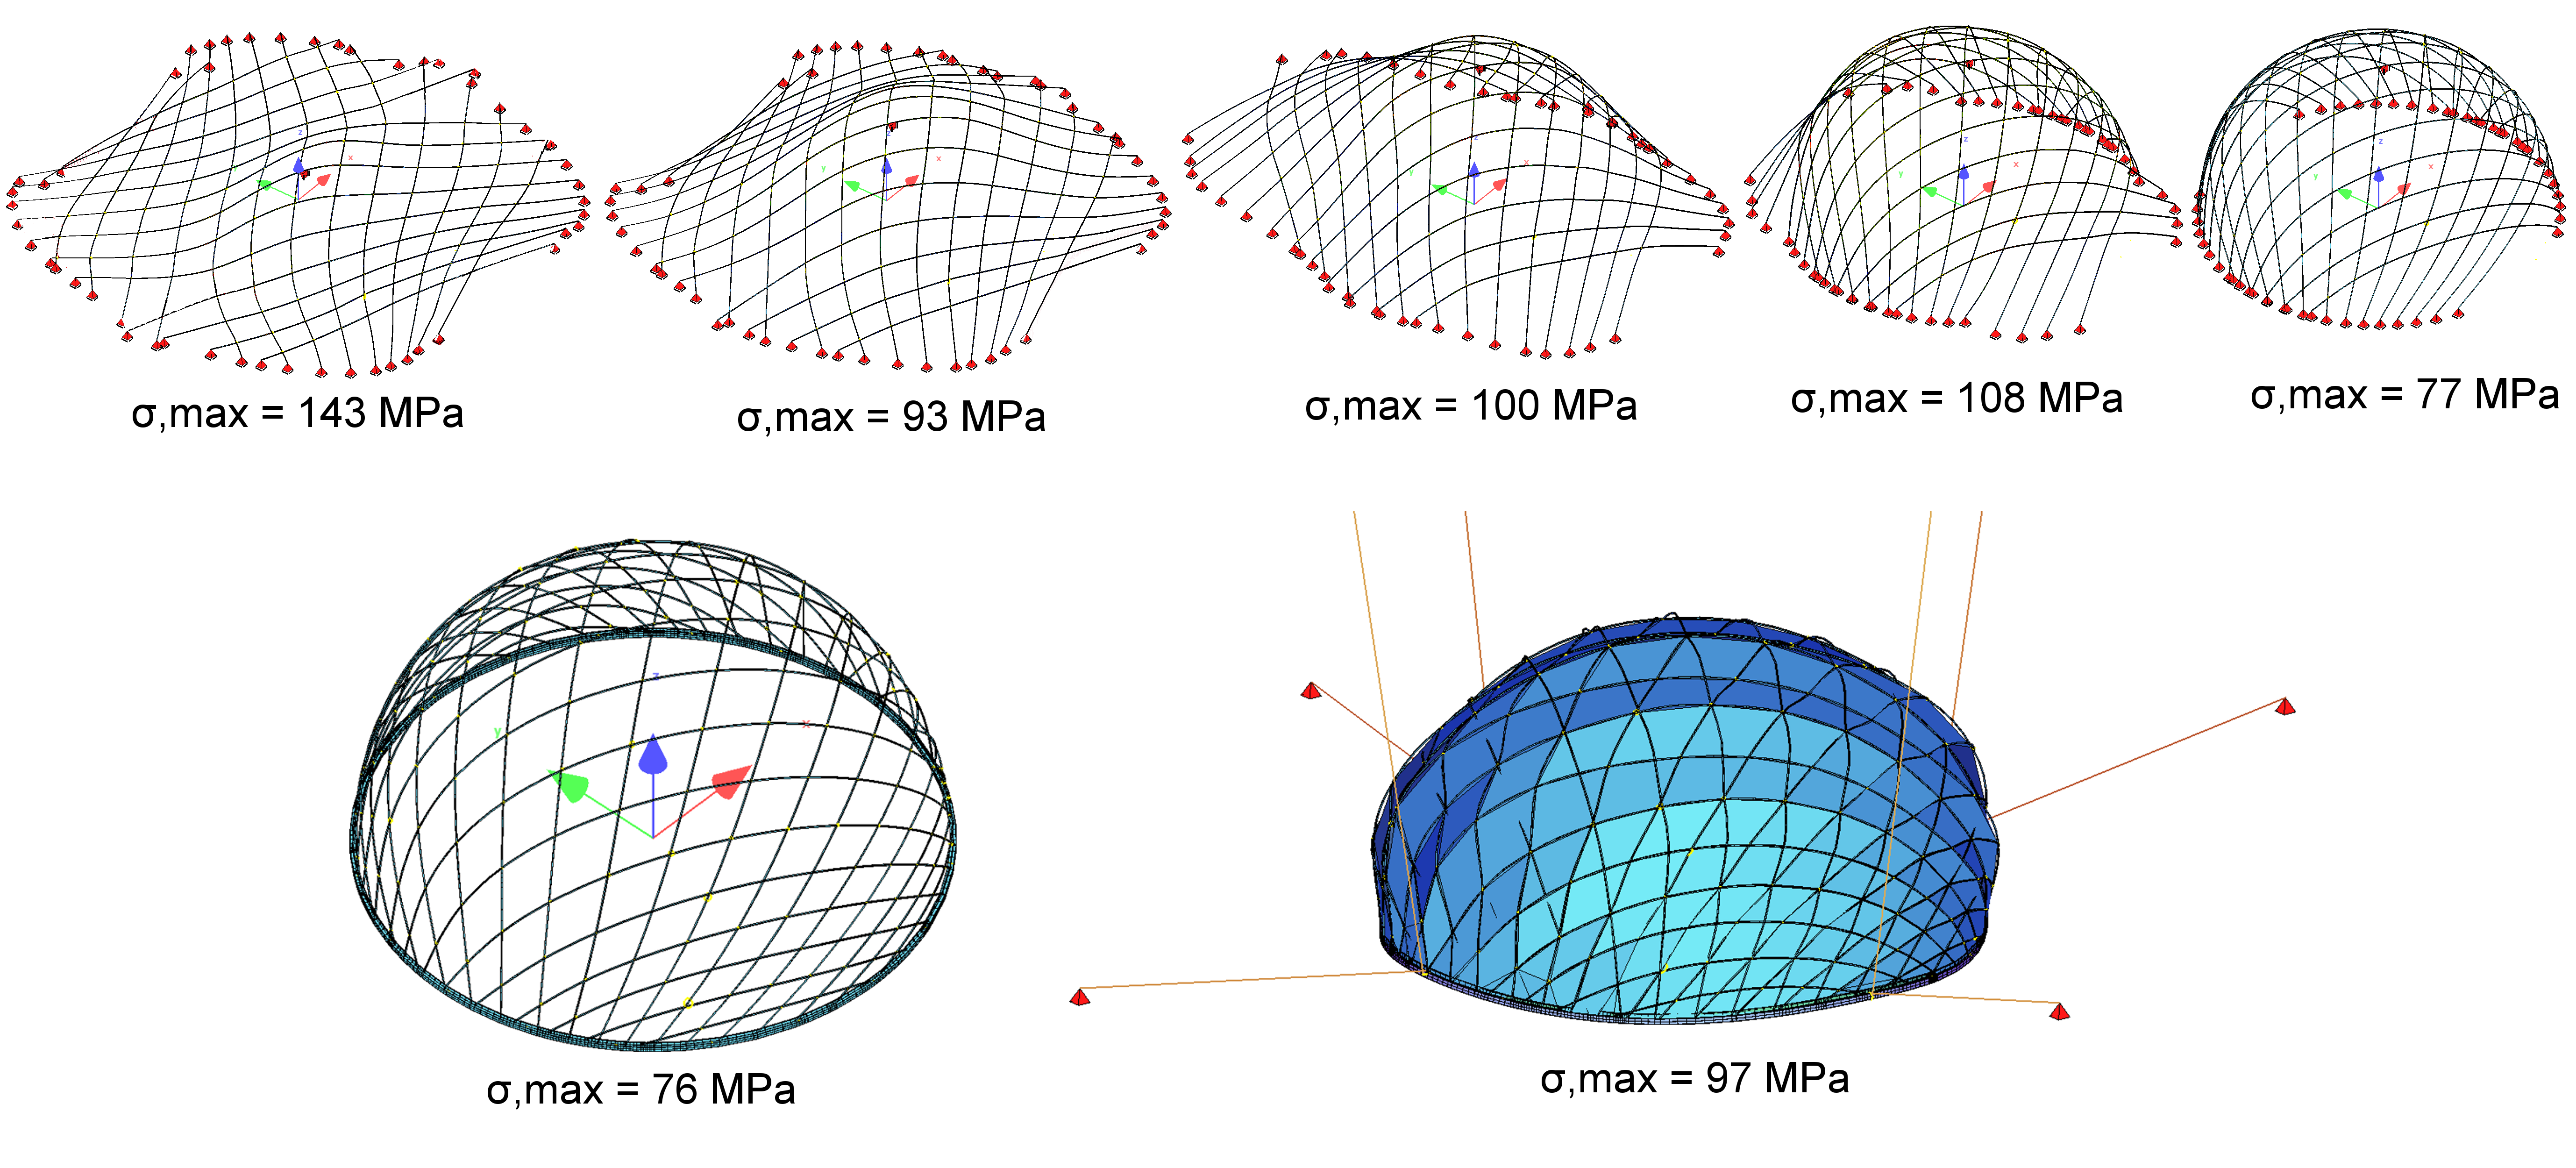
\includegraphics[width=1.0\linewidth]{images/CaseStudies_Irregular/FEMGlobal.png}
\caption{Simulation of the erection process and loading of the Flying Dome and analysis of the maximum stresses by means of FEA}
\label{fig:FEMGlobal}
\end{figure}








